\documentclass[11pt,paper=letter]{scrartcl}

\usepackage[wide]{cjquines}
\usepackage{graphicx}

\makeatletter
\def\fps@figure{htbp}
\makeatother

\begin{document}

\title{Pascal's theorem}

\author{Carl Joshua Quines}

\date{January 5, 2017}

\maketitle

\begin{abstract}
We set-up the projective plane (using plenty of pictures) to discuss Pascal's theorem. Three example problems are discussed, followed by a problem set.
\end{abstract}

\section{Motivation}

In the Euclidean plane we are familiar with, any two lines intersect at a point -- unless these lines are parallel. You probably are familiar with a theorem that has ``concurrent or all parallel'' as a conclusion, for example, the radical center:

\begin{theorem*}[Radical center]
Given three intersecting circles $\omega_1, \omega_2$ and $\omega_3$ with distinct centers $O_1, O_2$ and $O_3$, the common chords are either concurrent or all parallel.
\end{theorem*}

\begin{figure}
  \centering
    \begin{minipage}{0.4\textwidth}
    \centering
    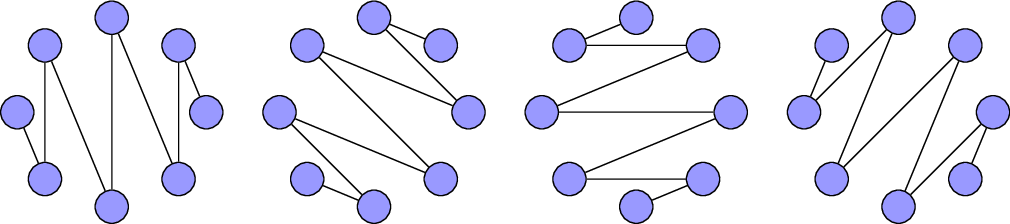
\includegraphics[width=\textwidth]{diagrams/1.pdf}
    \end{minipage}
    \begin{minipage}{0.4\textwidth}
    \centering
    \includegraphics[width=\textwidth]{diagrams/1b.pdf}
    \end{minipage}
  \caption{Left: concurrent. Right: all parallel.}
\end{figure}

By failing to consider an ``all parallel'' case, you can lose points. The language is clumsy, because two lines intersect at any point, unless they're parallel. If we could set parallel lines as intersecting in a certain pont, we could get rid of this condition.

We can't just let parallel lines intersect at a certain point, however. If this point is one of our regular points, then the lines wouldn't become parallel anymore. If the parallel lines did intersect, they must be at a new point \emph{outside} of the regular plane. Also, three lines that are parallel to each other should intersect at the same point, so ``all parallel'' can be replaced with ``concurrent''.

By adding these conditions to the Euclidean plane carefully, we create a new plane called the \emph{real projective plane}. We'll discuss the properties of the real projective plane by looking at art.

\subsection{Drawing in perspective}

How do artists represent three-dimensional items on a two-dimensional piece of paper? The way it works in theory is that if you have a three-dimensional object, place a sheet of paper in front of it, and draw lines from your eye to the object, you'd have a two-dimensional representation of something three-dimesnional.

Take the figure below as an example. We have a sheet of paper between our eyes on the top and a three-by-three board below. We draw lines from the eye to the three-by-three board and see where it intersects with the sheet of paper, which creates a \emph{projection} from the three-dimensional object to the two-dimensional sheet of paper. This is where we get the name projective from.

\begin{figure}
\centering
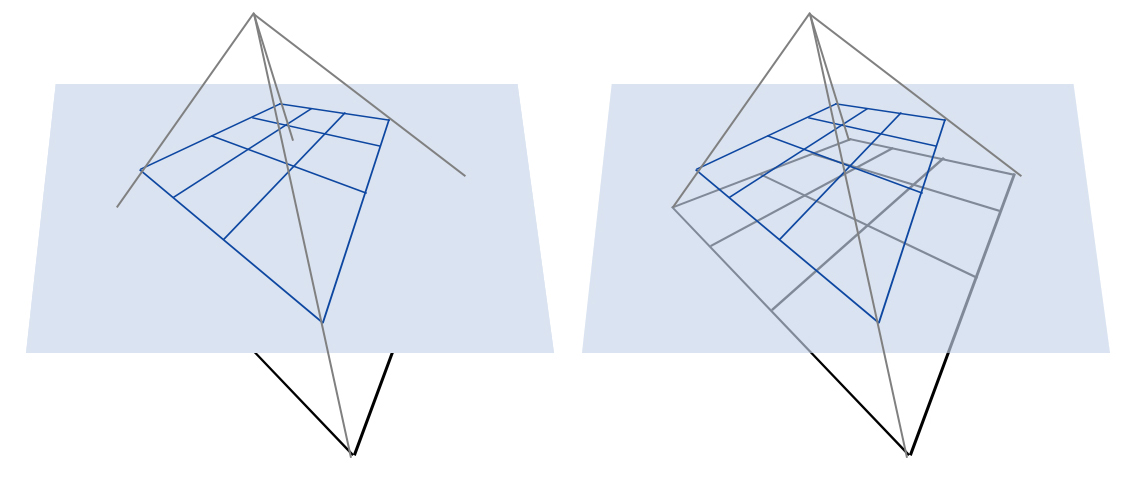
\includegraphics[width=\textwidth]{projection.jpg}
\caption{Projecting a three-by-three board to a sheet of paper.}
\end{figure}

Now, the new figure on the sheet of paper is a representation of the three-by-three board. Although it is quite a stretch from what it would look like if we looked at the board straight-on from above, it is similar to what it would look like if we placed the board near our eye level.

Below are two different ways to draw the same board. We just drew one figure from one perspective and the other figure from another perspective. As a consequence, we can position these two drawings in three dimensions so they look the same -- just use the above projection to the sheet of paper.

\begin{figure}
\centering
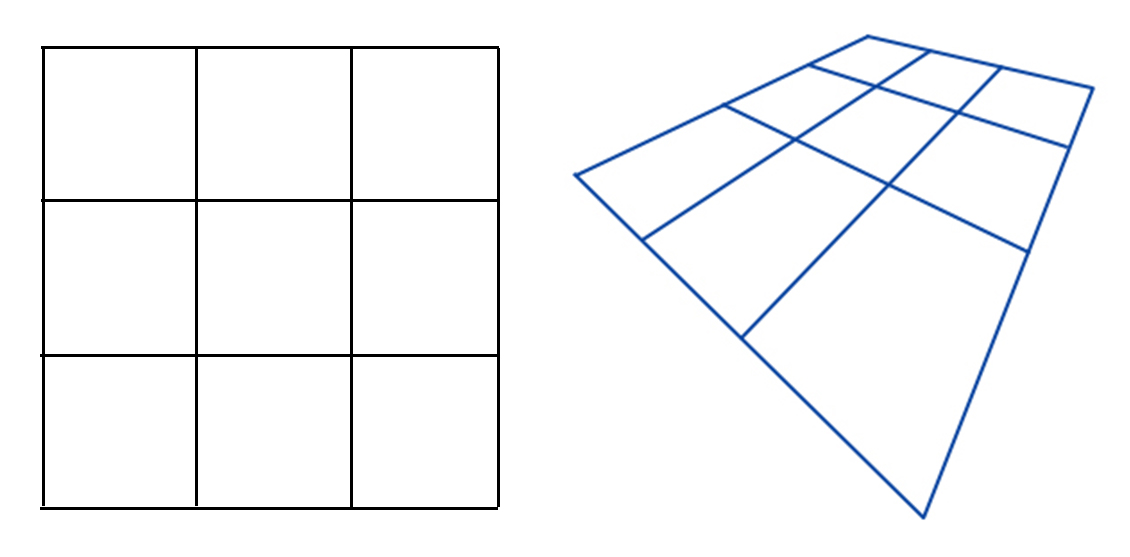
\includegraphics[width=3in]{twothreebythree.jpg}
\caption{Two ways to look at the same board.}
\end{figure}

Let's look at what happens to the parallel lines. In the left figure, we already see two sets of parallel lines: the horizontal lines, which are all parallel, and the veritcal lines, which are also all parallel. But if you look at the right figure closely, the parallel lines from the left figure suddenly aren't parallel. They intersect at two different points.

In fact, there's two more sets of parallel lines in the first figure. The diagonals of the squares in the first figure have to be parallel as well, giving us two more sets of lines which are parallel. In the right figure, the supposedly parallel diagonals also intersect at a point.

\begin{figure}
\centering
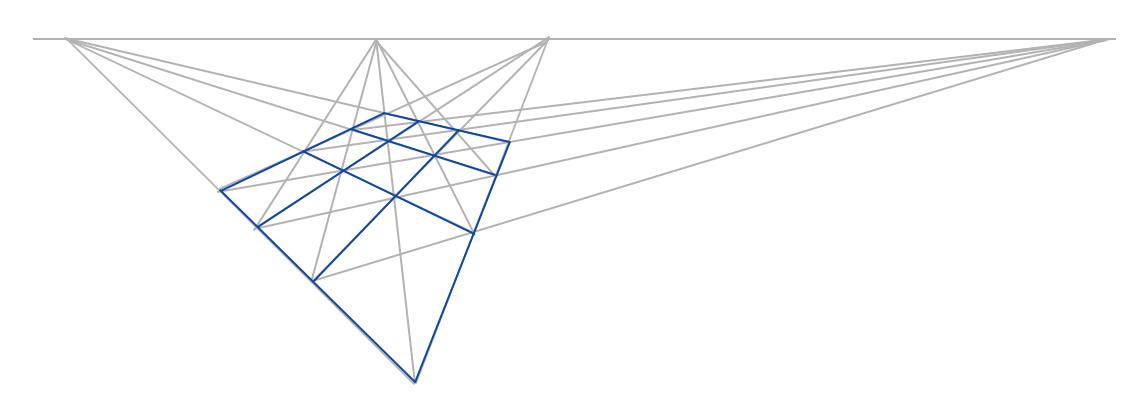
\includegraphics[width=\textwidth]{two-point.jpg}
\caption{Parallel lines intersect.}
\end{figure}

If we draw all the points where these supposedly parallel lines intersect, we can notice that they all lie on a single line. Suddenly our parallel lines intersect -- and what's more, their intersections all lie on a single line.

The \emph{real projective plane} takes this idea and formalizes it. We have the regular points of the Euclidean plane, which are called \emph{Euclidean points}. Parallel lines \emph{do} intersect, at points we call \emph{points at infinity}. Each parallel line in the same direction concurs at the same point. Finally, there's an extra line called the \emph{line at infinity}, the line which all the points at infinity lie on.

Looking at the above figure gives us an idea of what the real projective plane looks like. All the parallel lines in the original three-by-three board intersect (at infinity), and the intersections are all colllinear (at the line at infinity). What was all parallel in the original three-by-three board is now concurrent (at infinity) at the real projective plane! Now we can avoid the iffy language of ``concurrent or all parallel'' and just replace it with ``concurrent''.

\section{Pascal's theorem}

Now we can discuss Pascal's thoerem, whose natural setting is in the projective plane. We need some notation: we write the intersection of lines $AB$ and $CD$ as $AB \cap CD$, which can be points at infinity.

\begin{theorem*}[Pascal's theorem]
Let $ABCDEF$ be a hexagon inscribed in a conic, possibly self-intersecting. Then the points $AB \cap DE, BC \cap EF$ and $CD \cap FA$ are collinear.
\end{theorem*}

We call the common line the \emph{Pascal line}. Looking at Pascal's theorem, we immediately observe that it is a tool for collinearities and concurrences. It handles points on a conic and their intersections. A bunch of points all lying on the same circle with a bunch of intersections is a big hint for Pascal's.

Pascal's theorem can also look very different depending on what order the vertices are around the circle. A few examples are shown below.

\begin{figure}
  \centering
    \begin{minipage}{0.33\textwidth}
    \centering
    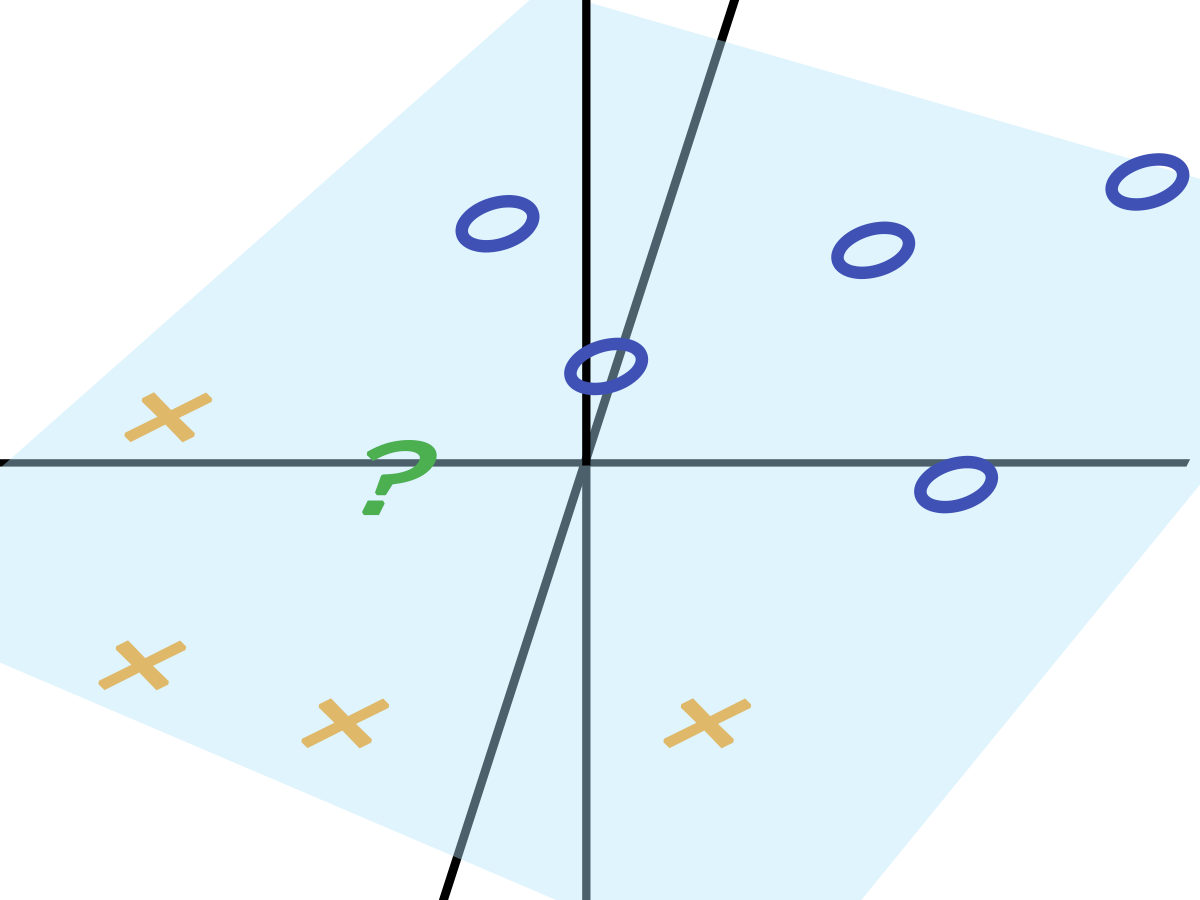
\includegraphics[width=\textwidth]{diagrams/2.pdf}
    \end{minipage}
    \begin{minipage}{0.33\textwidth}
    \centering
    \includegraphics[width=\textwidth]{diagrams/2a.pdf}
    \end{minipage}
    \begin{minipage}{0.33\textwidth}
    \centering
    \includegraphics[width=\textwidth]{diagrams/2b.pdf}
    \end{minipage}
    \begin{minipage}{0.33\textwidth}
    \centering
    \includegraphics[width=\textwidth]{diagrams/2c.pdf}
    \end{minipage}
  \caption{Pascal's can look very different.}
\end{figure}

Finally, a note on Pascal's before we start the example problems: we can degenerate a side of a hexagon to a single pont. The side $AA$, then, would become the tangnet to the conic at the point $A$. Think of this as the limit of the side $AB$ by making $A$ and $B$ closer and closer together.

\begin{figure}
  \centering
    \begin{minipage}{0.25\textwidth}
    \centering
    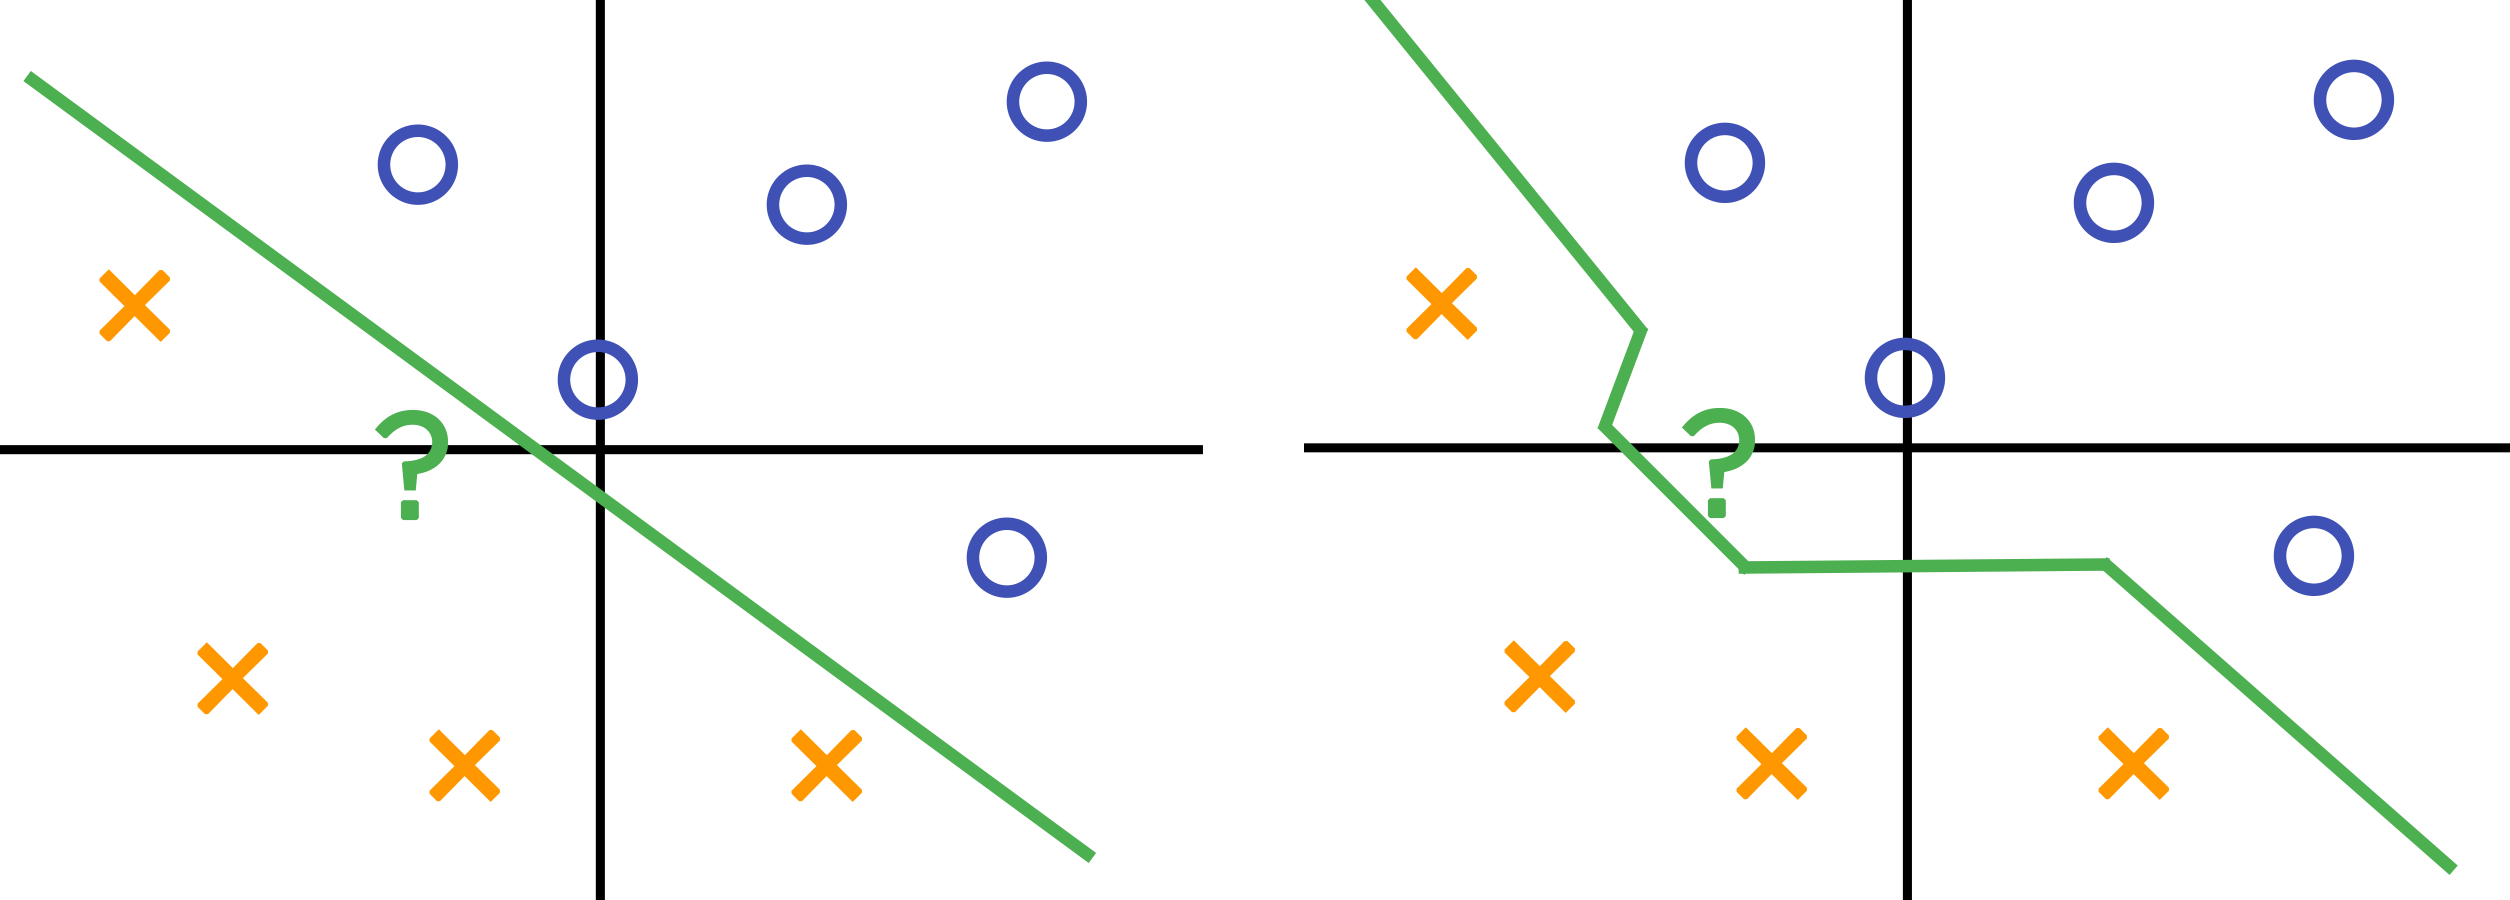
\includegraphics[width=\textwidth]{diagrams/3.pdf}
    \end{minipage}
    \begin{minipage}{0.3\textwidth}
    \centering
    \includegraphics[width=\textwidth]{diagrams/3a.pdf}
    \end{minipage}
    \begin{minipage}{0.3\textwidth}
    \centering
    \includegraphics[width=\textwidth]{diagrams/3b.pdf}
    \end{minipage}
  \caption{Degenerating $AB$ to $AA$.}
\end{figure}

\section{Example problems}

\begin{problem}
  Let $ABCD$ be a cyclic quadrilateral, let the tangents to $A$ and $C$ intersect in $P$, the tangents to $B$ and $D$ in $Q$. Let $R$ be the intersection of $AB$ and $CD$ and let $S$ be the intersection of $AD$ and $BC$. Show that $P,Q,R,S$ are collinear.
\end{problem}

\begin{figure}
\centering
    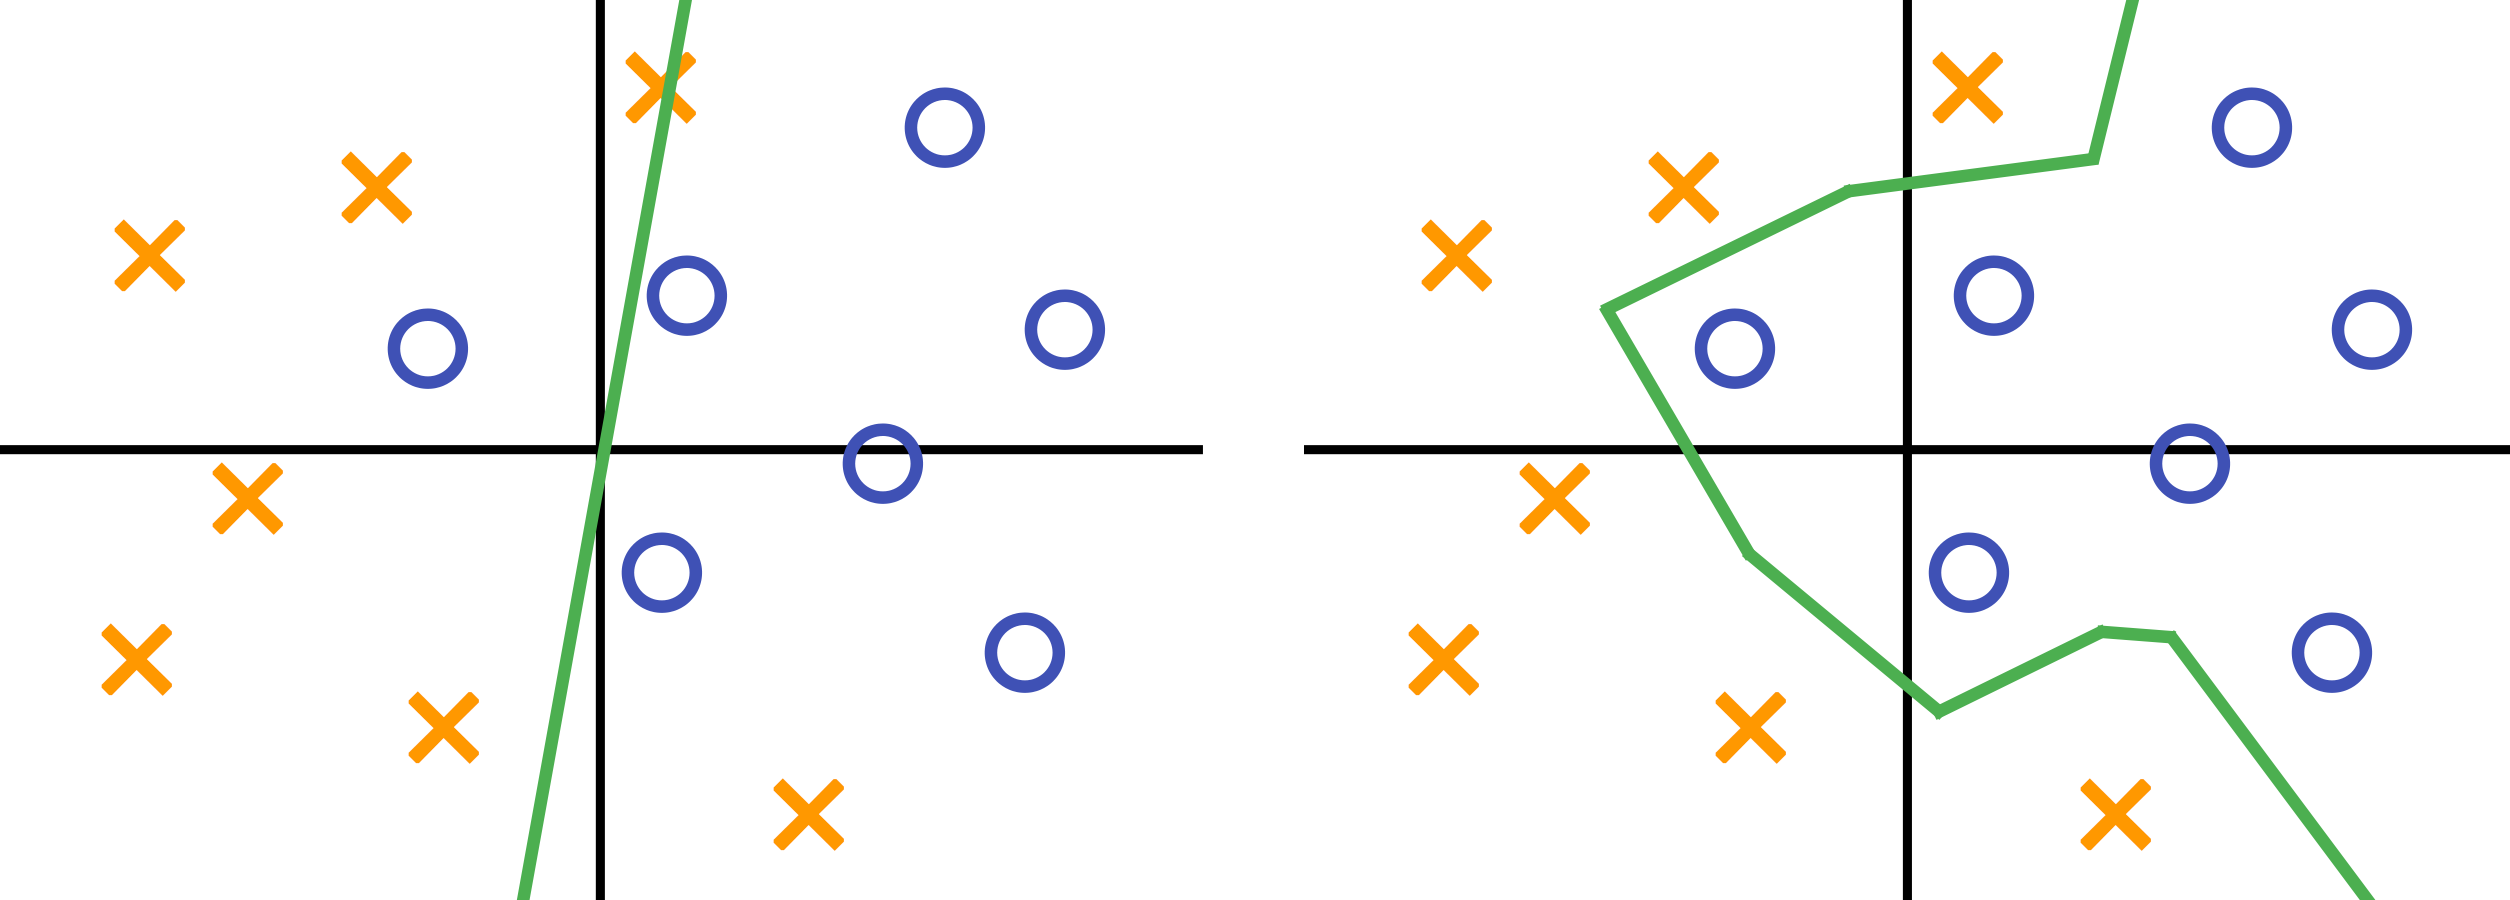
\includegraphics[width=2.5in]{diagrams/4.pdf}
\caption{Our first example problem.}
\end{figure}

What is our tip-off for Pascal's? The very prominent circumcircle of $ABCD$, as well as the multitudes of intersections based on points on this circle, tell us that using Pascal's might provide some information.

The first thing I do in a problem like this, where a projective solution might occur, is to represent points as intersections of lines. For example, I'd write $P = AA \cap CC$, as well as the other intersections $$Q = BB \cap DD, R = AB \cap CD, S = AD \cap BC.$$

If I want to use Pascal's to show three of these points are collinear, we'd have to pick one of these points as one intersection. Let's pick $P$, which is $AA \cap CC$. We fill $AA \cap CC$ as the first intersection for our hexagon, which so far looks like $AA\_CC\_$.

The second intersection, so far, is $A\_ \cap C\_$. We look at our points for something that follows this pattern, and we notice that $R$ follows it. $R$ is $AB \cap CD$, so we try filling in $B$ and $D$ for the blanks.

Now our hexagon looks like $AABCCD$. Using Pascal's gives us the third intersection, which is $BC \cap DA$. However, this is point $S$. Thus $P, R$ and $S$ are collinear. This is encouraging, and we look for another hexagon, and we see that $ABBCDD$ gives us $$AB \cap CD = R, BB \cap DD = Q, BC \cap DA = S,$$ so $Q, R$ and $S$ are collinear, which ends our proof. We write it up neatly:

\begin{proof}
  Using Pascal's on hexagon $AABCCD$ gives us $P, R$ and $S$ are collinear. Similarly, using Pascal's on hexagon $ABBCDD$ gives us $Q, R$ and $S$ are collinear. Thus $P, Q, R$ and $S$ are all collinear.
\end{proof}

From this problem we get our first two heuristics for Pascal's:

\begin{itemize}

\item Pascal's theorem is a tool for collinearities and concurrences. A bunch of points, all lying on the same circle, with a bunch of intersections is a hint for Pascal's, especially if we want to prove a collinearity or concurrence.

\item Often we want to find the points we wish to show collinear \emph{before} finding the hexagon. Then we write each point as the intersection of two lines with endpoints at the conic, and work backwards to find the hexagon.

\end{itemize}

We present another example that involves more than just working backwards, and this time from an actual olympiad.

\begin{problem}
  (Singapore TST) Let $\omega$ and $O$ be the circumcircle and circumcenter of right triangle $ABC$ with $\angle B = 90\dg$. Let $P$ be any point on the tangent to $\omega$ at $A$ other than $A$, and suppose ray $PB$ intersects $\omega$ again at $D$. Point $E$ lies on line $CD$ such that $AE || BC$. Prove that $P, O, E$ are collinear.
\end{problem}

\begin{figure}
\centering
    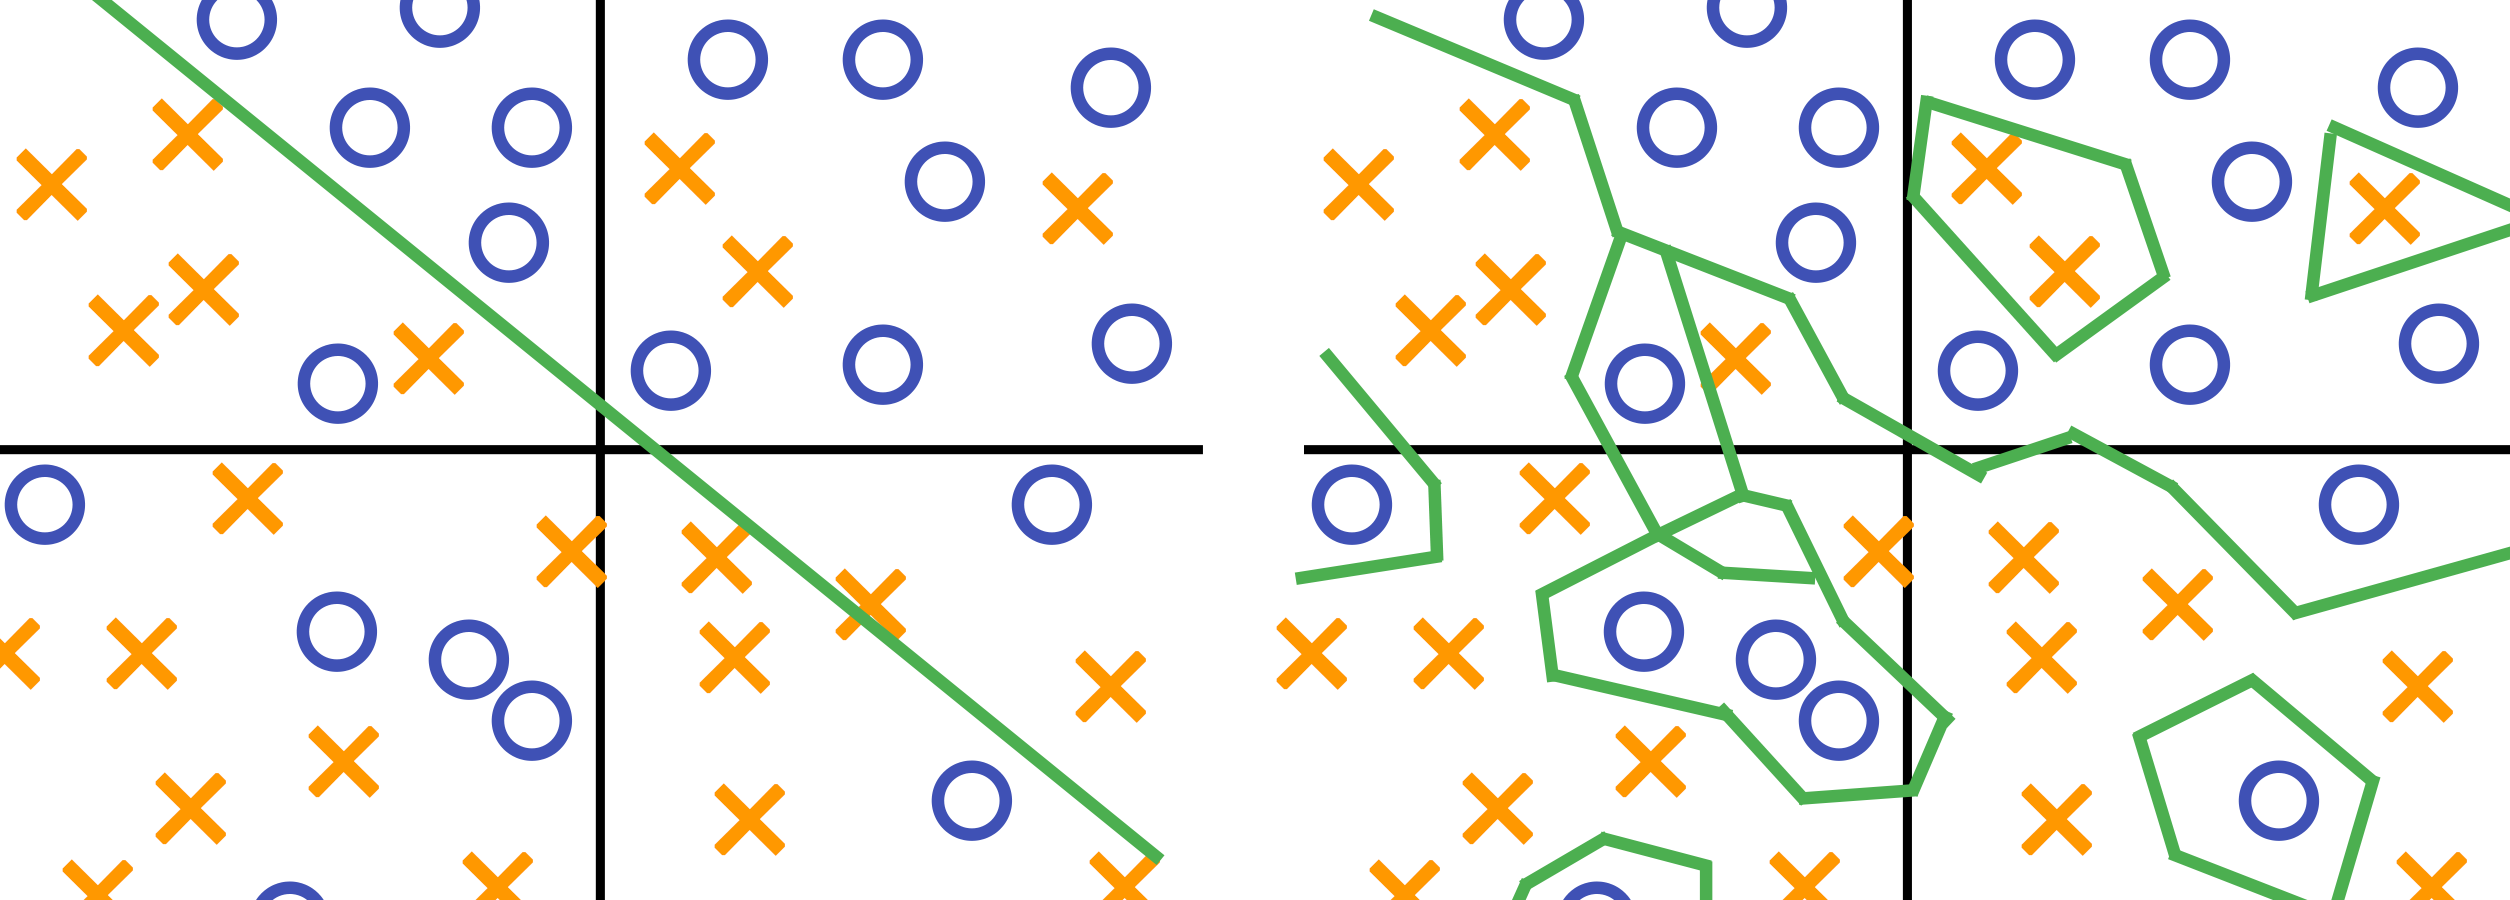
\includegraphics[width=2in]{diagrams/5.pdf}
\caption{A Singaporean TST.}
\end{figure}

Again, the tip-off for Pascal's is ``a bunch of points, all lying on the same circle, with a bunch of intersections.'' We want to prove $P, O$ and $E$ are collinear, using Pascal's. So let's write the points as intersections: $$P = AA \cap BD, O = AC \cap \ldots, E = DC \cap \ldots$$ Uh oh. We ran out of points. This means we have to add an additional point somewhere so we can get $O$ and $E$ down.

Where is this additional point? Let's try to use Pascal's right now. Taking $P$ as the first intersection, our hexagon so far is $AA\_BD\_$. We have $O$ lying on $AC$ and $E$ lying on $DC$, so to get both of these down we can try placing $C$ in the last spot, so our hexagon is $AA\_BDC$. (If we place $C$ in the middle spot, we'd get the segment $BC$, which none of our points lie on.)

Let's think. What are the lines with endpoints on the circle passing through $O$? They're the diameters. $AC$ is a diameter. In $AA\_BDC$, the intersection with $AC$ is~$\_B \cap AC$. If this has to be $O$, then $\_B$ has to be a diameter. The unknown point has to be the point that makes a diameter with $B$. Let's try naming this point $X$.

\begin{figure}
\centering
    \includegraphics[width=2in]{diagrams/5a.pdf}
\caption{Adding in diameter $BX$.}
\end{figure}

So $BX$ is a diameter, and $AAXBDC$ is our hexagon. The remaining intersection is $AX \cap DC$, which has to be $E$. We only need to show that $A, X$ and $E$ are collinear.However, recall the definition of $E$ as the point on $CD$ such that $AE||BC$. To show that $A, X$ and $E$ are collinear, we only need to show that $AX||BC$. But $ABCX$ is a rectangle, hence this is true, and we are done.

\begin{proof}
  Let $X$ be the point on circle $\omega$ such that $BX$ is a diameter. Since $ABCX$ is a rectangle, $AX||BC$, so $A, X$ and $E$ are collinear. Finally, using Pascal's on $AAXBDC$ gives us $P, O$ and $E$ as collinear.
\end{proof}

The point $X$ has a special name. It's the \emph{antipode} of $B$, the reflection of $B$ over the center of the circle. From this problem we get two more heuristics for using Pascal's:

\begin{itemize}

\item The center of a circle is the intersection of two of its diameters. If you're trying to prove that the center of a circle is collinear to two other points, involving two diameters can help.

\item Involving a diameter is often done by adding the antipodes of points. The antipode of a point $A$ is its reflection $A'$ over the center of the circle. Then $AA'$ passes through the center of the circle, and is a diameter.

\end{itemize}

Finally, we do an ISL problem, just to show the power of Pascal's.

\begin{problem}
  (ISL 2004/G2) Let $\Gamma$ be a circle and let $d$ be a line such that $\Gamma$ and $d$ have no common points. Further, let $AB$ be a diameter of the circle $\Gamma$; assume that this diameter $AB$ is perpendicular to the line $d$, and the point $B$ is nearer to the line $d$ than the point $A$. Let $C$ be an arbitrary point on the circle $\Gamma$, different from the points $A$ and $B$. Let $D$ be the point of intersection of the lines $AC$ and $d$. One of the two tangents from the point $D$ to the circle $\Gamma$ touches the circle at a point $E$; hereby we assume that the points $B$ and $E$ lie in the same half-plane with respect to the line $AC$. Denote by $F$ the intersection of the lines $BE$ and $d$. Let the line $AF$ intersect the circle $\Gamma$ at a point $G$ different from $A$. Prove that the reflection of the point $G$ in the line $AB$ lies on the line $CF$.
\end{problem}

\begin{figure}
\centering
    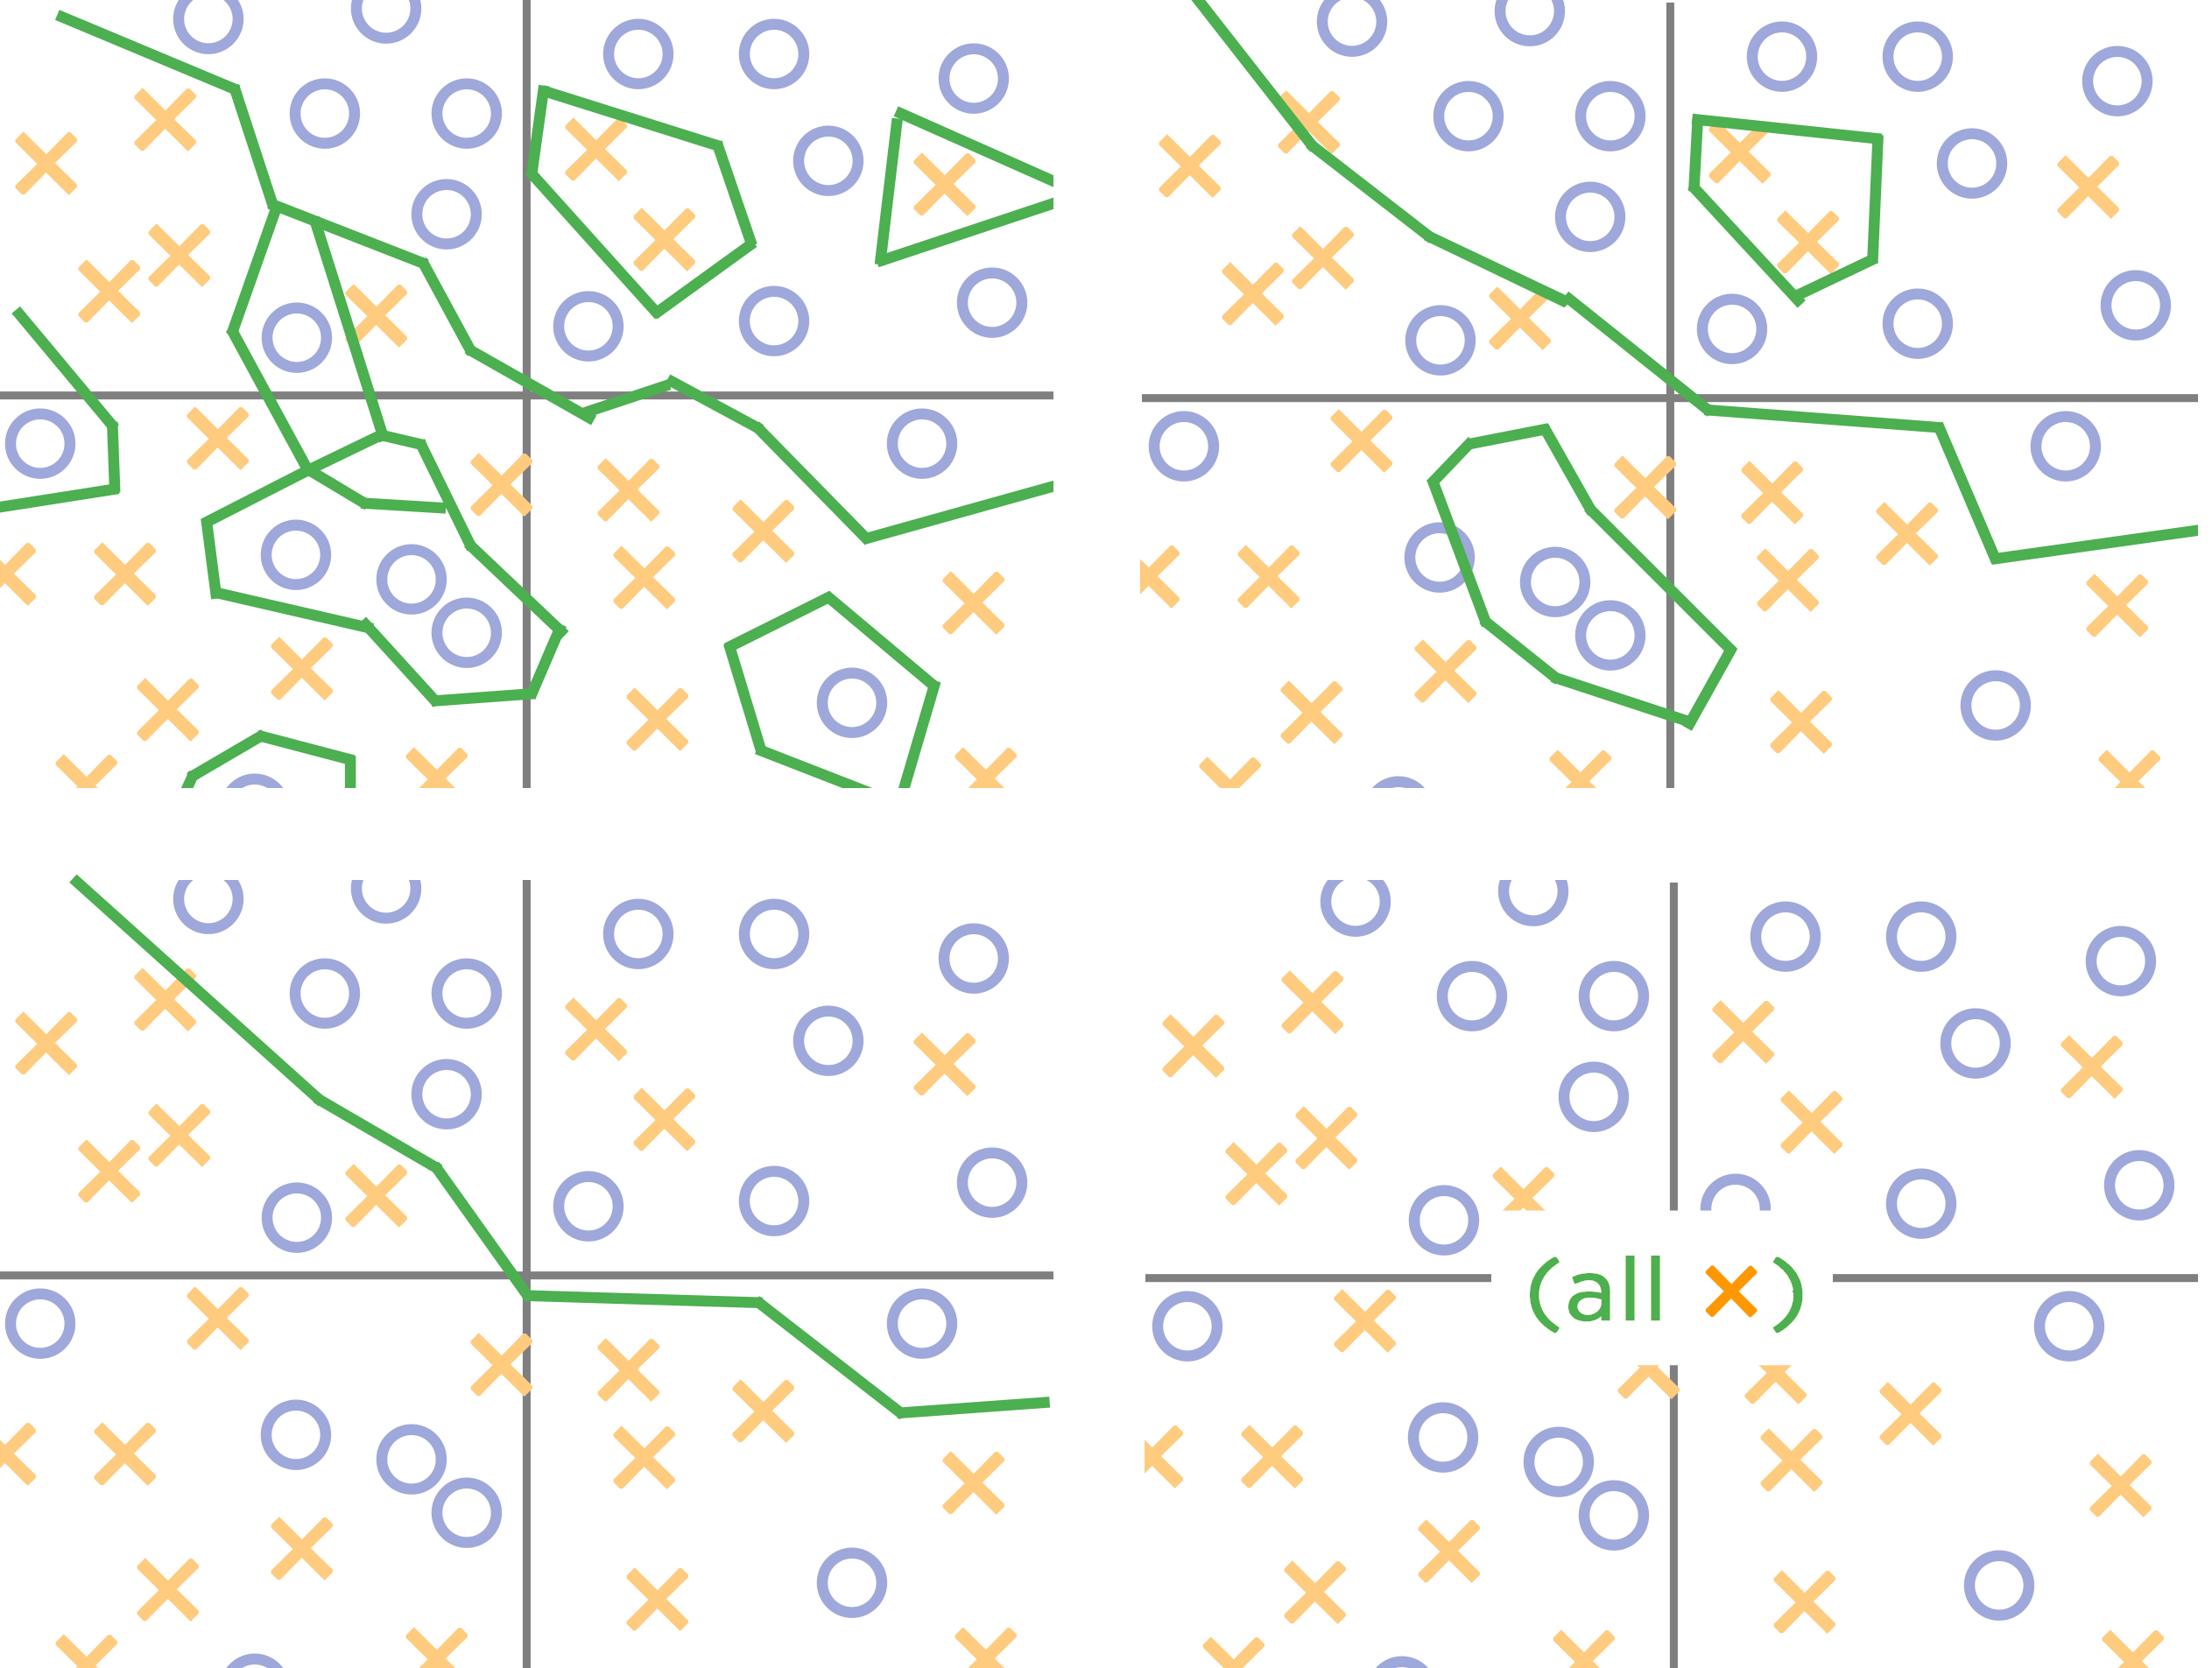
\includegraphics[width=2in]{diagrams/6.pdf}
\caption{An ISL G2.}
\end{figure}

Let's call the reflection of $G$ on $AB$ as $G'$. What is our tip-off for Pascal's? Again, there is a prominent circle which six points pass through, $A, G, C, B, E, G'$, and a lot of intersections involving these points.

We begin with the usual: $F = AG \cap BE$ and $D = AC \cap EE$. We want to show that $C, G'$ and $F$ are collinear. Our usual approach won't work here, since two of those points are on the circle.

Let's try using Pascal's on $F$ and $D$ to see if we can get any new points. We're motivated to do this because $F$ and $D$ have similar endpoints in the lines that define them. Starting with point $F$ gives us $AG\_BE\_$. Note that we can't insert $C$ and $E$ to get $AC \cap EE$, so we try again by switching $BE$ to $EB$.

Now our hexagon is $AG\_EB\_$, and we can insert $E$ in the first blank and $C$ in the second to get $AC \cap EE$. The hexagon is now $AGEEBC$ and the new point is $GE \cap BC$. This point lies on the line $d$ as well.

Now we have three points on the line $d$, $F, D$ and $GE \cap BC$. Somehow, we need to involve the segment $CG'$ to get $F$. Let's try fitting in $CG'$ and the new point $GE \cap BC$. Fill out the hexagon as $GE\_BC\_$, and add in point $G'$ to the second blank to get $GE\_BCG'$.

In hexagon $GE\_BCG'$, the third point, $\_B \cap G'G$, must also lie on $d$. The third point must be the intersection of $G'G$ and $d$. But these two lines are parallel, as $AB$ is perpendicular to $d$. So the third point must be on the line through $B$ parallel to $d$ -- which is tangent to $\Gamma$.

From this we see the first point must be $B$, so the hexagon is $GEBBCG'$. The third point is then $EB \cap CG'$, which must be on the line $d$. But the point on line $d$ that lies on $EB$ is $F$, so $EB \cap CG' = F$, and $C, G'$ and $F$ are collinear.

\begin{proof}
  Let $G'$ be the reflection of $G$ over $AB$. Pascal's theorem on $AGEEBC$ shows that $BC \cap GE$ lies on $d$. Applying Pascal's theorem again on $CG'GEBB$ means $CG' \cap BE$ lies on $d$, which means the intersection must be the point $F$, and thus $F$ lies on $CG'$.
\end{proof}

What motivated this solution? One possible reason would be the point $F$ -- we want to show that $$F = AG \cap BE \cap d \cap CG',$$ and if we have a point that lots of lines pass through, we try to involve it in Pascal's twice, getting the same line in the process. From this we get our final two heuristics:

\begin{itemize}
  \item If we fill out points and our first hexagon doesn't seem to fit, we can always try exchanging the letters. However, sometimes we have to do trial and error on lots of different hexagons.

  \item If we have a point that lots of lines pass through, we try to involve it in Pascal's twice and get the same line in the process. This can reveal new information about collinearities.
\end{itemize}

\section{Summary}

Here's a list of the heuristics we found for using Pascal's theorem:

\begin{itemize}

\item Pascal's theorem is a tool for collinearities and concurrences. A bunch of points, all lying on the same circle, with a bunch of intersections is a hint for Pascal's, especially if we want to prove a collinearity or concurrence.

\item Often we want to find the points we wish to show collinear \emph{before} finding the hexagon. Then we write each point as the intersection of two lines with endpoints at the conic, and work backwards to find the hexagon.

\item The center of a circle is the intersection of two of its diameters. If you're trying to prove that the center of a circle is collinear to two other points, involving two diameters can help.

\item Involving a diameter is often done by adding the antipodes of points. The antipode of a point $A$ is its reflection $A'$ over the center of the circle. Then $AA'$ passes through the center of the circle, and is a diameter.

\item If we fill out points and our first hexagon doesn't seem to fit, we can always try exchanging the letters. However, sometimes we have to do trial and error on lots of different hexagons.

\item If we have a point that lots of lines pass through, we try to involve it in Pascal's twice and get the same line in the process. This can reveal new information about collinearities.

\end{itemize}

Finally, a small tip. Pascal's is just one of the many tools to prove collinearity and concurrence. It plays well with other theorems like Ceva's and Menelaus's. It especially plays well with projective ones like Pappus's, Desargues's and Brianchon's.

\section{Problems}

While a lot of the problems can be solved without Pascal's, the solutions presented is where Pascal's theorem is a key step. Straightforward problems usually involve one or two applications, involved problems require a bit more ingenuity, while challenging problems are difficult enough to be olympiad problems and will often not require Pascal's alone. Problems are very roughly sorted by difficulty.

\subsection{Straightforward}

\begin{enumerate}

\item Let $ABCDEF$ be a hexagon inscribed in a circle such that $AB$ is parallel to $DE$ and $BC$ is parallel to $EF$. Prove that $CD$ and $AF$ are parallel.

\item Cyclic quadrilateral $ABCD$ is such that the tangents to the circle from $B$ and $D$ intersect at $AC$. Prove that the tangents to the circle from $A$ and $C$ intersect at $BD$.

\item (CTK \cite{CTK4}) Chords $AB$ and $CD$ are parallel, whereas $P$ and $Q$ are additional points on the same circle. Let $X$ be the intersection of $BP$ and $CQ$, $Y$ the intersection of $AQ$ and $DP$. Prove that $XY$ is parallel to $AB$ and $CD$.

\item Let $ABCD$ be a quadrilateral whose sides $AB, BC, CD, DA$ are tangent to a single circle at points $M, N, P, Q,$ respectively. Let lines $BQ, BP$ intersect the circle at $E, F$ respectively. Prove that lines $ME, NF, BD$ are concurrent.

\item (CTK \cite{CTK8}) Points $A,B,C$ lie on a conic, $D$ elsewhere. The conic meets $AD, BD, CD$ the second time in $A', B', C'$. $N$ is also on the conic. $A'N, B'N, C'N$ cross $BC, AC, AB$ in $A_0, B_0, C_0$. Prove points $A_0, B_0, C_0$ and $D$ are collinear.

\item Let $ABC$ be a triangle and let $B_1, C_1$ be points on the sides $CA, AB$. Let $\Gamma$ be the incircle of $ABC$ and let $E, F$ be the tangency points of $\Gamma$ with the same sides $CA$ and $AB$, respectively. Furthermore, draw the tangents from $B_1$ and $C_1$ to $\Gamma$ which are different from the sidelines of $ABC$ and take tangency points with $\Gamma$ to be $Y$ and $Z$, respectively. Prove that the lines $B_1C_1, EF,$ and $YZ$ are concurrent.

\end{enumerate}

\subsection{Involved}

\begin{enumerate}

\item Line $AB$ is tangent to circle $\omega$ at point $Y$, with $Y$ between $A$ and $B$ on the line. Point $X$ is on circle $\omega$ such that $XY$ is a diameter. Suppose $XA$ and $XB$ meet the circle again at $C$ and $D$, respectively, and that $AD$ and $BC$ meet the circle again at $E$ and $F$, respectively. Prove that $XE = XF$.

\item (Grinberg \cite{CTK3}) Given a cyclic quadrilateral $ABCD$ with the circumcenter $O$. The perpendicular to $BD$ through $B$ meets the perpendicular to $AC$ through $C$ at $E$. The perpendicular to $BD$ through $D$ meets the perpendicular to $AC$ through $A$ at $F$. Finally, let $X$ be the intersection of the lines $AB$ and $CD$. Prove the points $O, E, F, X$ are collinear.

\item (Steiner \cite{CTK1}) Prove that the Pascal lines of the hexagons $ABCDEF, ADEBCF,$ and $ADCFEB$ are concurrent.

\item (Kirkman \cite{CTK1}) Prove that the Pascal lines of the hexagons $ABFDCE, AEFBDC,$ and $ABDFEC$ are concurrent.

\item (Mellery \cite{CTK9}) A circle with center $O$ has $AB$ as a diameter. The arbitrary points $C$ and $D$ are on one semicircle so that arc $AC$ is within the arc $AD$. Pick an arbitrary point $E$ on the other semicircle. $I$ is the intersection of $CE$ with $AD$, $K$ is the intersection of $IO$ with $BE$. Prove that $\angle CDK = 90\dg$.

\item (CTK \cite{CTK5}) Given three points $P, Q, R$ and a circle. Choose a point $A$ on the circle and extend $AP$ to meet the circle in $B'$. Extend $B'Q$ to meet the circle in $C$. Extend $CR$ to meet the circle in $A'$. Extend $A'P$ to meet the circle in $B$. Extend $BQ$ to meet the circle in $C'$ and, finally, extend $C'R$ to meet the circle in $X$. Prove that $P, Q$ and $R$ are collinear if and only if $X$ and $A$ coincide.

\item (La Hire's theorem) Let $A, B, C, D, E$ and $F$ be points on the same circle. Let $X$ be the intersection of the tangents from $A$ and $D$, $Y$ be the intersection of the tangents from $B$ and $E$, and $Z$ be the intersection of the tangents from $C$ and $F$. Prove that $X, Y$ and $Z$ are collinear if and only if $AD, BE$ and $CF$ concur.

\end{enumerate}

\subsection{Challenging}

\begin{enumerate}

\item (APMO 2013/5) Let $ABCD$ be a quadrilateral inscribed in a circle $\omega$, and let $P$ be a point on the extension of $AC$ such that $PB$ and $PD$ are tangent to $\omega$. The tangent at $C$ intersects $PD$ at $Q$ and the line $AD$ at $R$. Let $E$ be the second point of intersection between $AQ$ and $\omega$. Prove that $B$, $E$, $R$ are collinear.

\item (Nikolin \cite{CTK7}) Let $ABC$ and $DEF$ be two triangle inscribed in the same circle. Their sides intersect in six points $G,H,I,J,K,L$. ($G = AB \cap FE, H = AB \cap DF, I = BC \cap DF, J = BC \cap DE, K = DE \cap CA, L = EF \cap CA$) Prove that the lines $GJ, HK,$ and $IL$ are concurrent.

\item (CTK \cite{CTK6}) Let $O$ be the center of a circle with diameters $BB_t, CC_t$ and $M_tN_t$ and chords $BA_b$ and $CA_c$. Assume that $BA_b$ intersects $M_tN_t$ in $M$ and $CA_c$ intersects $M_tN_t$ in $N$. $K_b$ is the second point of intersection of $NB_t$ with the circle. $K_c$ is the second point of intersection of $MC_t$ with the circle. Prove that $A_b$ and $A_c$ coincide if and only if so do $K_b$ and $K_c$.

\item $A$ is a point not on the circle $\omega$ and $M$ and $N$ are on $\omega$ such that $AM,AN$ are tangent to it. Line $x$ passes through $M$ and cuts $AN$ at $P_{1}$ and line $y$ passes through $N$ and cuts $AM$ at $P_{2}$. $P_{1}P_{2}$ intersects $MN$ at $S$. The tangent at the second intersection of $x$ and $\omega$ intersects $AM$ at $T$ and The tangent at the second intersection of $y$ and $\omega$ intersects $AN$ at $R$. Prove that $S,T$ and $R$ are collinear.

\item (ELMO Shortlist 2012/A10) Let $A_1A_2A_3A_4A_5A_6A_7A_8$ be a cyclic octagon. Let $B_i$ by the intersection of $A_iA_{i+1}$ and $A_{i+3}A_{i+4}$. (Take $A_9 = A_1$, $A_{10} = A_2$, etc.) Prove that $B_1, B_2, \ldots , B_8$ lie on a conic.

\item Triangle $ABC$ has incenter $I$, circumcircle $\omega$ and circumcenter $O$. The circle with diameter $AI$ intersects $\omega$ again at $Q$. Let $N$ be the midpoint of arc $BAC$. Let the line tangent to $\omega$ passing through $A$ intersect $QN$ at another point $M$. Prove that $M, I$ and $O$ are collinear.

\item (ISL 2007/G5) Let $ABC$ be a fixed triangle, and let $A_1, B_1, C_1$ be the midpoints of sides $BC, CA, AB,$ respectively. Let $P$ be a variable point on the circumcircle. Let lines $PA_1, PB_1, PC_1$ meet the circumcircle again at $A', B', C'$ respectively. Assume that the points $A, B, C, A', B', C'$ are distinct, and the pairwise intersections of lines $AA', BB', CC'$ form a triangle. Prove that the area of this triangle does not depend on $P$.

\end{enumerate}

\section{Hints}

\subsection{Straightforward}

\begin{enumerate}

\item This is not that hard.

\item List down the points as intersections of lines passing through two points in the circle, and search for something that can use Pascal's.

\item Proving that $XY$ is parallel to $AB$ and $CD$ is the same as showing they all concur at infinity.

\item Use Pascal's as well as Brianchon's.

\item The challenge is finding the right hexagons. Be organized!

\item Don't consider $ABC$ as the main triangle, consider $\Gamma$ as the main circle.

\end{enumerate}

\subsection{Involved}

\begin{enumerate}

\item $XE = XF$ is not a collinear or concurrence condition, but it can be made into one. How?

\item How do we involve the center of the circle in Pascal's?

\item Use Desargues's.

\item Use Desargues's too.

\item The line through $I, O$ and $K$ looks suspiciously like a Pascal line.

\item What is the Pascal line?

\item A proof using only Desargues's and Pascal's is possible.

\end{enumerate}

\subsection{Challenging}

\begin{enumerate}

\item Use the second problem from the Straightforward list.

\item Use Pascal's and trig Ceva.

\item What is the Pascal line?

\item List down the points of intersection and try to use Pascal's.

\item Recall that Pascal's is an ``if an only if'', so Pascal's converse is also true.

\item Point $O$ looks so disconnected. How can we involve it? We also need to use a certain well-known lemma.

\item The fact that this problem appears in this handout is already a big hint. Use the fact that the area of a triangle is $\frac{1}{2}ab \sin C$.

\end{enumerate}

\begin{thebibliography}{99}

\bibitem{CTK1} Pascal Lines: Steiner and Kirkman Theorems. Available at \url{http://www.cut-the-knot.org/Curriculum/Geometry/PascalLines.shtml}

\bibitem{CTK3} Pascal in a Cyclic Quadrilateral. Available at \url{http://www.cut-the-knot.org/Curriculum/Geometry/PascalInQuadrilateral.shtml}

\bibitem{CTK4} Parallel Chords Entail Another Parallel. Available at \url{http://www.cut-the-knot.org/Curriculum/Geometry/ParallelChords.shtml}

\bibitem{CTK5} Pascal: Necessary and Sufficient. Available at \url{http://www.cut-the-knot.org/Curriculum/Geometry/PascalIterations.shtml}

\bibitem{CTK6} Diameters and Chords. Available at \url{http://www.cut-the-knot.org/Curriculum/Geometry/DiametersAndChords.shtml}

\bibitem{CTK7} Two Triangles Inscribed in a Conic. Available at \url{http://www.cut-the-knot.org/Curriculum/Geometry/GeoGebra/Steiner_Pascal.shtml}

\bibitem{CTK8} Two Pascals Merge into One. Available at \url{http://www.cut-the-knot.org/m/Geometry/DoublePascalConic.shtml}

\bibitem{CTK9} Surprise: Right Angle in Circle. Available at \url{http://www.cut-the-knot.org/m/Geometry/RightAngleInCircle.shtml}

\end{thebibliography}

If anyone knows the sources to any problem without one, see an error, have a correction, or have a question, please do not hestitate to contact me at \mailto{cj@cjquines.com}.

\end{document}
